\documentclass[12pt,a4paper]{report}

\usepackage[utf8]{inputenc}
\usepackage[T1]{fontenc}
\usepackage{lmodern}
\usepackage{titlesec} 
\usepackage{graphicx}
\usepackage{microtype}
\usepackage{hyperref} 
\usepackage{amssymb}
\usepackage[frenchb]{babel}
\usepackage{listings}
\usepackage{amsmath}
\usepackage{enumitem}
\usepackage{float} 

\usepackage{pict2e}

\usepackage{listings}	  

\lstdefinestyle{customstyle}{
    basicstyle=\footnotesize,
    breakatwhitespace=false,         
    breaklines=true,                 
    captionpos=b,                    
    keepspaces=true,                                                                                       
    tabsize=4,
    frame=single,
    moredelim=[is][\underbar]{_}{_}
}
\lstset{style=customstyle}

\title{Projet de recherche}
\author{Antoine Forgerou \and Jérémy Bardon \and Nicolas Bourdin}
\date{}

% Permet de masquer les affichages de "Chapitre" 
\titleformat{\chapter}[hang]{\bf\huge}{\thechapter}{2pc}{} 
\begin{document}
	\renewcommand{\contentsname}{Sommaire}
	\maketitle	

	\tableofcontents	
	\newpage
	
	\setlength{\unitlength}{1cm}
	
	
\chapter{Introduction}
Ce document est un rapport rassemblant le travail effectué dans le cadre du module 
d'initiation à la recherche au sein du Master 1 ALMA. Ce module permet d'initier 
les étudiants au travail de recherche en informatique. 
\\\\
Le sujet de recherche auquel nous avons contribuer est le suivant : 

\begin{center}
	  \textbf{Modélisation et analyse des systèmes logiciels hétérogènes}
\end{center}

La préoccupation de l'équipe est de trouver un moyen d'assurer la cohésion d'un système
hétérogène lors d'opérations d'ajout et/ou de suppression des modèles le composant. 
Tout les modèles seront alors capables de communiquer ensembles et dans un premier temps, 
le choix a été fait de s'appuyer sur l'exemple d'automates que l'on voudrait composer.
\\\\
Au cours de ce rapport, différents points seront abordés. Tout d'abord une 
présentation du laboratoire LINA ainsi que l'équipe AeLoS que nous avons intégré le 
temps du module de recherche. Nous reviendrons alors plus en détail sur la 
problématique soulevée par le sujet pour ensuite présenter les 3 solutions proposées
par l'équipe. Ensuite, nous expliquerons la solution que nous avons choisi de mettre 
en place et nous rentrerons au cœur du projet avec la présentation de la solution
que nous avons implémenter.	

\chapter{Présentation du laboratoire}
Acteur central du développement de l'informatique dans la région des Pays de La Loire, le LINA (Laboratoire d'Informatique de Nantes Atlantique) est un laboratoire de recherche en sciences et technologies du logiciel qui est dirigé par Pierre Cointe. Avec ses 180 membres, ce laboratoire est actuellement situé sur deux sites Nantais : la Lombarderie (Faculté des Sciences et Techniques) et la Chantrerie (Ecole des Mines et Polytech' Nantes).


\section{Les différentes équipes}
Le LINA est composé des équipes suivantes : 
\begin{itemize}
  \item AeLoS : \textbf{A}rchitecture et \textbf{Lo}giciel \textbf{S}ûrs
  \item ASCOLA : \textbf{AS}pect and \textbf{CO}mposition \textbf{LA}nguages
  \item AtlanMod : \textbf{Atlan}tic \textbf{Mod}eling 
  \item COD : \textbf{CO}nnaissances et \textbf{D}écision
  \item ComBi : \textbf{Com}binatoire et \textbf{Bi}oinformatique
  \item DUKe : \textbf{D}ata \textbf{U}ser \textbf{K}nowledg\textbf{e}
  \item GDD : \textbf{G}estion de \textbf{D}onnées \textbf{D}istribuées
  \item GRIM : \textbf{G}estion, \textbf{R}ésumé, \textbf{I}nterrogation, et apprentissage sur les \textbf{M}asses de données
  \item OPTI : Optimisation globale, optimisation multi-objectifs
  \item TALN : \textbf{T}raitement \textbf{A}utomatique du \textbf{L}angage \textbf{N}aturel
  \item TASC : Programmation par contraintes
\end{itemize}

\chapter{L'équipe AeLoS}	

L'équipe AeLoS, dirigé par Christian ATTIOGBE, est une équipe de recherche intégrée au LINA résultant de la fusion de deux anciennes équipes COLOSS et MODAL.

Le projet central de cette équipe s'appuie sur les trois thématiques suivantes :
\begin{itemize}[label=$\circ$]
  \item Architecture : 
  \item Composants logiciels corrects : 
  \item Multiformalisme et analyse multifacette : 
\end{itemize}

\section{Les membres}
Une récente liste des membres est disponible sur le site du LINA, à l'adresse suivante : \\
\url{http://www.lina.univ-nantes.fr/spip.php?page=membres&id_equipe=15&lang=fr}
\chapter{Présentation du sujet}


\section{Problématique}

\paragraph*{Contexte}: Approches formelles des systèmes embarqués communiquants.\\

La construction rigoureuse d'un logiciel se fait à partir de son modèle. Pour des 
logiciels complexes (par exemple ceux qui ont de nombreux composants différents -- 
hétérogènes-- et qui communiquent), on dispose de plusieurs modèles (hétérogènes 
aussi) qui doivent intérargir de façon cohérente, pour garantir l'interopérabilité 
sémantique entre les modèles puis les composants logiciels. Le domaine des systèmes 
embarqués (et aussi des objets connectés) regorge d'exemples.\\

\paragraph*{Description du travail}: Etudier l'interopérabilité entre des modèles de composants (logiciels ou non).\\
En nous appuyant dans un premier temps sur des modèles à base d'automates à états, il s'agit dans le cadre du stage
d'initiation à la recherche, de contribuer à la conception et au développement d'outils passerelle entre modèles.\\\\

Nous travaillons sur plusieurs aspects :\\
\begin{itemize}
  \item Lorsque cela est possible, en fonction de la sémantique des modèles, un modèle donné est encodé par un autre
modèle choisi mais qui est sémantiquement équivalent.
  \item Lorsque cela est possible, en fonction de la sémantique des modèles, un modèle peut interagir avec un autre avec
des contrats (de type Assume/Guarantee)
  \item Plug'N'Check (analyse systématique de modèles/composants)
  \item etc
\end{itemize}

\section{Solutions proposées par l'équipe AeLoS}\label{sec:Solutions}
Pour répondre à la problématique, l'équipe AeLoS nous a proposé 3 façons de 
faire tout en nous laissant la liberté d'en proposer d'autres.
\\\\
Dans le but de simplifier les exemples, nous avons fait le choix de représenter 
les modèles comme des formes géométriques que l'on essayerais d'emboiter.
\\\\
La première solution consiste à adapter un des modèles au deuxième quand cela 
est possible. On peut prendre l'exemple du théorème de Kleene qui assure qu'un 
automate à états finis peut être écrit sous la forme d'une expression 
rationnelle et vice et versa.

\begin{figure}[h]
	\centering
	
\includegraphics[scale=1]{ressources/solution1.png}
	\caption{Solution 1 - Adaptation d'un modèle}
\end{figure}

Dans cet exemple c'est le composant de gauche qui s'est adapté pour pouvoir intéragir
avec la partie droite.
\newpage
L'approche qui parait la plus évidente mais qui peut se révéler complexe 
consiste à intégrer un troisième modèle dans le système. Ce dernier va alors 
jouer le rôle de passerelle entre les deux modèles que l'on veut faire 
communiquer.

\begin{figure}[h]
	\centering
	
\includegraphics[scale=1]{ressources/solution2.png}
	\caption{Solution 2 - Interface entre les modèles}
\end{figure}

Plug'N'Check est le nom de la troisième solution que l'équipe nous a soumise. 
Le principe est de faire interagir les modèles ensemble puis d'effectuer des 
vérifications pour déterminer si les modèles peuvent communiquer à 100\%, 
en partie ou pas du tout.

\begin{figure}[h]
	\centering
	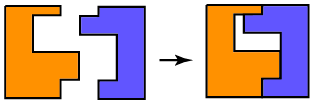
\includegraphics[scale=1]{ressources/solution3.png}
	\caption{Solution 3 - Plug'N'Check}
\end{figure}

L'exemple montre que certaines parties sont satisfaites mais d'autres parties ne 
peuvent pas communiquer.
\\\\
Dans le cadre de notre stage d'initiation à la recherche, nous nous sommes 
orientés vers la première solution. Nous avons donc entrepris de transformer 
n'importe quel modèle dans un language commun afin de permettre de les 
interfacer.
\\\\
Il est admis que les automates sont des une spécialisation de graphe, ce qui 
signifie que n'importe quel automate peut-être repésenté sous forme de graphe. 
C'est la raison qui nous a poussé à utiliser le language \emph{DOT} 
\newpage
\section{Rappel sur les Automates}

    Les automates sur lesquels nous nous appuierons pour ce projet sont les automates à états fini, non-déterministe contenant des $\epsilon$-transistions.\\
    
    Rappelons la définition de l’automate à états fini non déterministe :
\begin{enumerate}
    \item un ensemble fini d’états, souvent noté Q 
    \item un ensemble fini de symboles, appelé alphabet et souvent noté $\Sigma$ 
    \item une fonction de transition, souvent nommée $\delta$, qui reçoit comme arguments un état de Q et un symbole de $\Sigma$ ou la chaîne vide notée $\epsilon$ et qui rend comme résultat une partie de Q \begin{center}$\delta : Q * ( \Sigma \cup \epsilon ) \rightarrow P(Q)$ \end{center}
    \item un état initial q0, appartenant à Q
    \item un sous-ensemble F de Q constitué des états finals, ou états acceptants\\
\end{enumerate}    


    Voici un exemple d'automate, extrait de notre projet :\\

\begin{figure}[h]
	\centering
	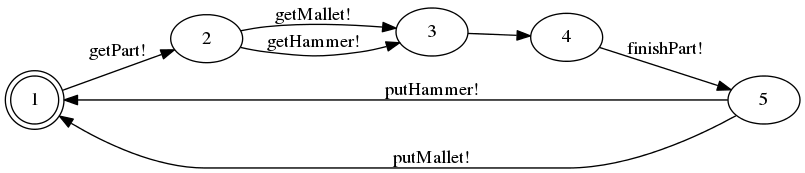
\includegraphics[scale=0.5]{ressources/img.png}
	\caption{Automate du jobber}
\end{figure}

\section{UPPAAL : un outil de modelisation des automates}
UPPAAL est un environnement intégré d'outils pour la modélisation , la validation et la vérification des systèmes temps réel modélisés comme des réseaux d' automates.
\\\\
Uppaal se compose de trois parties principales: 
\begin{itemize}[label=$\circ$]
  \item{ un langage de description}
  \item{ un simulateur}
  \item{ un vérificateur de modèle}
\end{itemize} 


  Le langage de description est un langage de commande non-déterministe avec des types de données (par exemple des entiers , des tableaux, etc. ) . Il se sert de la modélisation ou du langage de conception pour décrire le comportement du système grâce à des réseaux d'automates étendus avec des variables d' horloge et des données .\\ 

  Le simulateur est un outil de validation qui permet l'examen de possibles exécutions d'un système au début de la conception( ou la modélisation ) et fournit un moyen peu coûteux de détection de défaut avant la vérification par le vérificateur de modèle qui couvre l'ensemble des comportement dynamique du système.\\

  Le modèle orthographique peut vérifier les propriétés invariantes et l'accessibilité en explorant l'espace et l'état d'un système, c'est à dire l'analyse de l'accessibilité en termes d'états symboliques représentés par des contraintes .

\section{Le format DOT}

  Le langage DOT est un langage de description de graphe dans un format texte. C'est une manière simple de décrire des graphiques que les humains et les programmes informatiques peuvent utiliser. Les graphes DOT sont généralement des fichiers avec pour extension un .gv (ou .dot ).\\

  La syntaxe DOT peut aussi bien décrire des graphes non-orientés que des graphes orientés, comme des automates finis.
  Il est possible de placer des labels sur les transistions pour par exemple leurs donner un nom ou une explication. Le language possède aussi des attributs permettant une description graphique plus poussée, par exemple choisir la couleur d'un noeud ou de dessiner une transition en pointillé.

\subsection{Graphe non-orienté}

\begin{lstlisting}
graph monGraphe {
    a -- b -- c;
    b -- d;
}
\end{lstlisting}

  \textit{Resultat : }

\begin{figure}[!h]
  \centering
  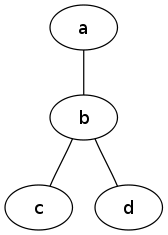
\includegraphics[scale=0.3]{ressources/grapheNO.png}
\end{figure}

\subsection{Graphe orienté}

\begin{lstlisting}
graph monGraphe {
    a -> b -> c;
    b -> d;
}
\end{lstlisting}

\begin{figure}[!h]
  \centering
  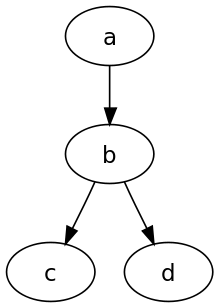
\includegraphics[scale=0.3]{ressources/grapheO.png}
\end{figure}

\newpage
\chapter[Hetersys : notre solution]{Hetersys\footnote{Heterogeneous systems: Tiré du nom du sujet de recherche "Modélisation et analyse des systèmes logiciels hétérogènes"} : notre solution}
\section{Introduction}

Notre but est de pouvoir composer n'importe quel type d'automate à l'aide du logiciel 
UPPAAL. Celui-ci propose de créer des automates et de les rassembler sous forme de projets 
mais il faut obligatoirement dessiner ces automates avec les outils mis à disposition.
\\\\
Etant donné que les automates sont un sous-ensemble des graphes, ce logiciel propose 
d'importer directement un automate -- décrit sous forme de graphe -- dans un projet 
UPPAAL pré-existant. 

\begin{figure}[h]
  \centering
  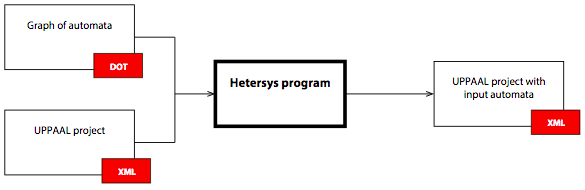
\includegraphics[scale=0.7]{ressources/ProgramScheme.png}
  \caption{Entrées et sorties du programme}
\end{figure}

Pour la description du graphe, nous avons choisi de nous appuyer
sur le format DOT bien connu qui est selon nous un langage très simple et minimaliste 
qui permet de construire des graphes très rapidement.

\section{Architecture logicielle}

L'architecture interne du programme a été pensée pour être la plus modulaire possible 
ce qui signifie que l'on peut facilement importer et/ou exporter dans un autre format
sans changer ce qui existe déjà. 
\\\\
En effet, le programme possède une représentation interne de l'automate sous forme 
de graphe ce qui rend ce genres d'ajustements plus simples. Les parties \emph{importer}
et \emph{exporter} constituent donc les points d'extension de notre programme.

\begin{figure}[!h]
  \centering
  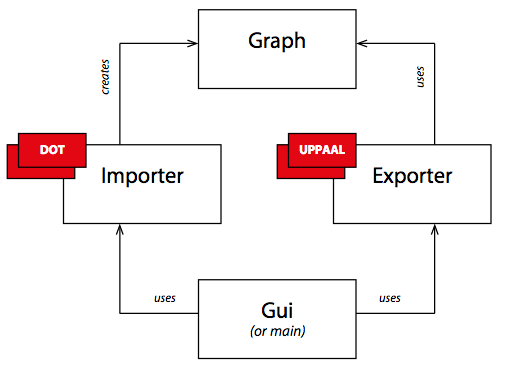
\includegraphics[scale=0.6]{ressources/archi.png}
  \caption{Composants du logiciel}
\end{figure}

Nous avons mis à disposition une interface graphique mais nous l'avons conçue dans l'optique 
de la découplée le plus possible du moteur de l'application. Il serait alors aisé de la supprimer
ou de la remplacer puisqu'elle suit le patron de conception MVC. 
\\\\
Par conséquent, la routine principale du programme ce trouve au niveau du 
\emph{modèle} qui se charge de dérouler le programme tout en interagissant 
avec l'interface.

\section{Fonctionnement interne}

La partie principale du programme est celle qui connaît et utilise l'importeur 
et l'exporteur. Le fonctionnement ce résume donc à utiliser ces deux composants
afin de charger l'automate et de l'ajouter dans le projet UPPAAL tout en procédant
à certaines vérifications au préalable.

\begin{figure}[!h]
  \centering
  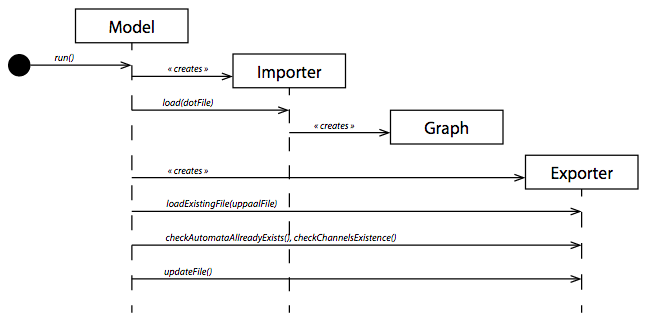
\includegraphics[scale=0.6]{ressources/deroulement.png}
  \caption{Schéma du déroulement du programme (non formalisé)}
\end{figure}

La ressource la plus importante est le graphe car il est généré par l'importeur 
puis utilisé par l'exporteur -- non représenté mais passé à la création -- pour 
vérifier la compatibilité avec le projet UPPAAL et la conversion dans le bon format.
\\\\
Par ailleurs, au niveau de l'implémentation -- avec l'interface graphique -- nous 
avons découpé cette routine en étapes. Ceci nous a permis de pouvoir reprendre 
à n'importe quel moment si il y a eu un souci et que l'utilisateur est en moyen de 
le résoudre via l'interface.
\\\\

\section{Choix techniques}
\subsection*{Technologie}
Nous avons décidé d'utiliser la technologie JAVA pour développer notre 
solution car il s'agit celle qui a été utilisé par les développeurs du projet UPPAAL.
\\\\
Celui-ci n'est pas open source mais s'il le devient ce sera alors plus facile d'intégrer
notre solution d'import directement en interne.

\subsection*{Aspect mis de coté}
Afin de nous concentrer sur la conversion du graphe et l'importation dans le projet UPPAAL,
le logiciel ne prend pas en compte la disposition graphique des éléments de l'automate.
\\\\
Il se contente alors de les afficher en ligne afin de pouvoir les identifier facilement mais 
l'utilisateur devra les réorganiser lui-même sachant que UPPAAL n'intègre pas de fonctions de 
réorganisation automatique

\section{Documentation du logiciel}
\subsection{Fenêtre principale}

Il s'agit du premier élément auquel l'utilisateur est confronté mais l'interface a été 
pensée pour faciliter l'apprentissage.

\begin{figure}[!h]
  \centering
  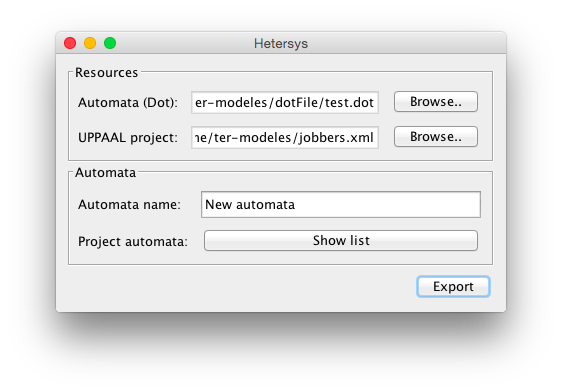
\includegraphics[scale=0.6]{ressources/gui/home.png}
  \caption{Fenêtre principale}
\end{figure}

En effet elle est décomposée en 2 parties: \emph{Resources} et \emph{Automata}. 
\\\\
La première partie regroupe les fichiers dont le programme à besoin en entrée à savoir 
un automate -- décrit sous forme de graphe en DOT -- et un projet UPPAAL pré-existant.
\\\\
La seconde section s'intéresse à l'automate qui sera ajouté dans le projet. Dans un projet
UPPAAL, chaque automate a un nom pour pouvoir l'identifier de manière unique ce qui veux 
dire que deux automates ne peuvent pas avoir le même nom. C'est pourquoi le bouton 
\og{}Show list\fg{} permet d'afficher le nom des automates déjà présents dans le projet 
afin de ne pas les réutiliser.
\\\\
Un appui sur le bouton export permet simplement d'exporter l'automate -- au format DOT -- 
dans le projet UPPAAL donné.

\subsection{Gestion des canaux}

L'automate donné en entrée n'ayant pas de contraintes particulières -- si ce n'est respecter 
le format DOT -- il n'est pas obligatoire que celui-ci ai des canaux en commun avec 
les autres automates du projet.
\\\\
C'est pourquoi, le logiciel va se charger de scanner les canaux utilisés dans l'automate 
et dans le projet pour notifier l'utilisateur dans 2 cas particuliers.

\subsubsection*{Canaux non déclarés}

Dans le cas où l'automate en entrée utiliserait des canaux qui ne sont pas déclarés
dans le projet UPPAAL, le logiciel demandera à l'utilisateur s'il veux les importer.

\begin{figure}[h]
  \centering
  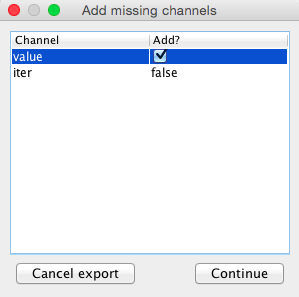
\includegraphics[scale=0.6]{ressources/gui/channels.png}
  \caption{Ajout de canaux}
\end{figure}

La liste des canaux permet de décider au cas par cas quel canaux il faut importer ou pas.

\subsubsection*{Aucun canaux en commun}
Le but de ce logiciel étant de composer les automates entre eux, lorsque l'automate en 
entrée n'a aucun canal en commun avec ceux dans le projet un message d'alerte apparaît.

\begin{figure}[h]
  \centering
  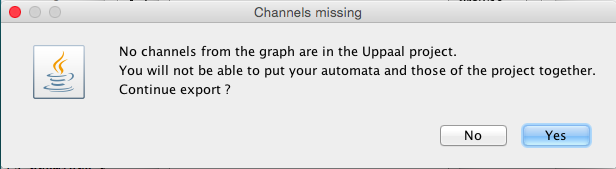
\includegraphics[scale=0.6]{ressources/gui/missing.png}
  \caption{Aucun lien entre les automates}
\end{figure}

Ceci permet à l'utilisateur d'annuler l'export pour changer son automate et utiliser 
des canaux déjà existants avant de le ré-exporter.

\subsection{Messages d'information}
\subsubsection*{Automate en double}
L'automate à insérer ne doit pas porter le même nom que ceux déjà dans le projet donc
une fenêtre notifie l'utilisateur si c'est le cas.

\begin{figure}[h]
  \centering
  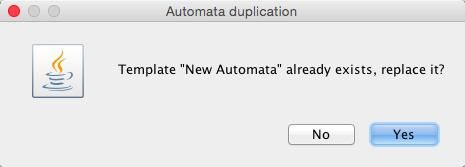
\includegraphics[scale=0.6]{ressources/gui/exists.png}
  \caption{Automate en double}
\end{figure}

\subsubsection*{Fin de l'export}
L'export d'un automate est très rapide mais le logiciel notifie quand même 
l'utilisateur quand celui-ci est terminé. 

\begin{figure}[h]
  \centering
  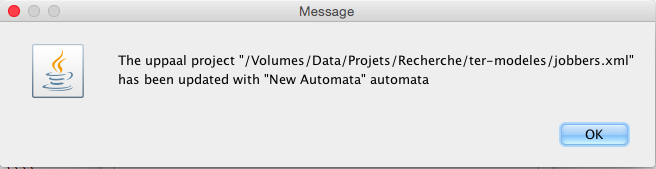
\includegraphics[scale=0.6]{ressources/gui/success.png}
  \caption{Export réussi}
\end{figure}

Le message rappelle quel projet UPPAAL a été modifié pendant l'opération mais 
aussi le nom de l'automate qui a été ajouté.

\section{Bilan}
\subsection{Résulats}
Après avoir étudié les 3 solutions proposées par l'équipe AeLoS (section \ref{sec:Solutions}) pour composer des systèmes hétérogènes, 
nous avons choisi de nous concentrer sur la première qui repose sur le principe d'adaptation.
\\\\
En effet, pour faire communiquer 2 automates de nature différente on peux essayer d'en modifier un 
pour qu'il s'adapte -- dans sa forme -- au second. Nous avons donc implémenté une solution reposant sur 
le logiciel UPPAAL qui lui propose de composer des automates entre eux.
\\\\
Notre solution -- appelée Hetersys -- permet d'importer un automate décrit sous forme de graphe -- au format DOT --
dans un projet UPPAAL qui contient d'autres automates. L'adaptation de l'automate se fait donc de manière naturelle
-- par le passage au format graphe -- et ce car n'importe quel type d'automate peux être représenté sous cette forme.

\subsection{Perspectives}
Si l'on se ressitue au niveau du problème dans sa globalité, notre outil permet de gérer l'ajout de composants logiciels
dans un système hétérogène mais il n'intègre pas encore toutes les éléments liés à cette opération. 
\\\\
Cela s'explique par le fait que la recherche sur le sujet n'est pas finie, elle demande donc plus de travail pour identifier
les points qui doivent être vérifiés lors de l'ajout -- ou de la suppression -- d'un modèle au sein d'un système hétérogène.
\\\\
Notre travail peut tout de même constituer une base pour tester des hypothèses sur le sujet et éventuellement  -- au travers
d'évolutions -- être un support pour démontrer par des expérimentations les résultats de la recherche.

\end{document}
